\section{Lossless Compression}

\subsection{Lempel-Ziv-Storer-Szymanski Algorithm}
Lempel-Ziv-Storer-Szymanski (LZSS)~\cite{storer1982data} is a lossless textual
compression algorithm.  It is a derivative and improvement of
LZ77~\cite{ziv1977universal} which  compressed data by using previous data as
dictionary. There is a sliding window and a look-ahead buffer applied in both
algorithms. Figure~\ref{fig:LZSS} shows the structure of LZSS. In LZ77
compression algorithm, a match between look-ahead buffer and dictionary is
encodes by which called \texttt{length-distance pair} (offset, length) where
offset is the distance from the first char of look-ahead and first char of the
match alphabet sequence~\cite{ziv1977universal}, e.g. (2, 3). For instance, a
alphabet sequence "AABCBABCD" shell be encoded to "(0, 0)A(1, 1)B(0, 0)C(2,
1)A(4, 2)D"  by using LZ77 compression method.
The problems of LZ77 method are: (1) When there is possible that the length of
coding result is longer than original match sequence. In last example, the first
A is encoded to (0, 0)A, but the extra length-distance pair is useless and needs
more bits to record it. (2) The single literal in coding result and following
literals might compose a longer match sequence to improve compression result.
For example, the third A in above example could combine following "BC" to make
up a longer sequence "ABC". 

LZSS solves these problems by defining a parameter \emph{MIN\_LENGTH} to
guarantee the size of the coding result is not larger than original sequence and
only output the pair ($n$, $m$), where $n$ indicates the offset, $m$ is the
length of the matching sequence~\cite{storer1982data}, rather than ($n$, $m$)$C$
in LZ77, where $C$ is the first character after longest matching sequence. The
compression process is shown as follow:

\begin{enumerate}
    \item Find the longest string $str$ which also appears in sliding
    window (dictionary) in look-ahead buffer.
    \item Compute offset $n$ and length $m$
    \item Check if the length $m$ is bigger or equals MIN\_LENGTH. If True, it
    outputs length-distance pair and data stream goes forward length of $str$,
    else outputs the first character in look-ahead buffer and stream goes
    forward 1 byte(character).
\end{enumerate}

For instance, assuming that the sliding window and look-ahead buffer are
unlimited, and that MIN\_length = 2,  string $aaBccDaacEaccFacac$ is encoded to
$aaBccD$(1, 2)$cE$(8, 2)$cF$(8, 2)(8, 2). LZSS is as simple as LZ77 for
compression and decompression, and the coding result is the only thing we needed
for decoding according (It is need not to send dictionary to client side).

\begin{figure}
    \centering
    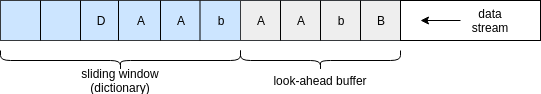
\includegraphics[width=\textwidth]{figures/LZSS.png}
    \caption{Structure of LZSS}
    \label{fig:LZSS}
\end{figure}

\subsection{Accelerometer-Lempel-Ziv-Storer-Szymanski Algorithm}
Accelerometer-LZSS~\cite{pope2018accelerometer} is a lossless, dictionary
compression algorithm based on LZSS. As we know, LZSS was introduced for textual
compression, but Pope et al.~\cite{pope2018accelerometer} implemented LZSS for
the devices with limited memory, storage and power. The authors compressed
accelerometer data using A-LZSS which combines LZSS and entropy coding (Huffman
code used in~\cite{pope2018accelerometer}). A flag bit is assigned to indicate
that either an entropy code or a length-distance pair $(n, m)$ is applied to
encoding. 

The pseudo-code of A-LZSS compression algorithm is shown in
Algorithm~\ref{algo:A-LZSS}. The function \texttt{longest\_match()} returns the
$D$ which donates the distance from cursor (the first symbol of look-ahead
buffer) to the first symbol of the match sequence, and the length $L$ of longest
matching sequence in buffer and dictionary~\cite{pope2018accelerometer}. In line
21 and 22 of Algorithm~\cite{pope2018accelerometer}, the $D-1$ and $L-1$ are
written in to bit stream rather than $D$ and $L$, since $D$ and $L$ can not be
0. It might save one bit to record the value $2^n$, for instance, three bit is
enough to record the number 8, and the subtracted 1 will be added back in
decompression process.

\begin{algorithm}
\begin{algorithmic}[1]
\Input
    \Desc{$symbols$}{$\quad \quad \quad \quad \quad \quad $Byte stream}
    \Desc{$L\_bits$}{$\quad \quad \quad \quad \quad \quad $number of bits for look-ahead buffer}
    \Desc{$D\_bits$}{$\quad \quad \quad \quad \quad \quad $number of bits for dictionary}
    \Desc{$minimum\_match$}{$\quad \quad \quad \quad \quad \quad $Minimum length of match sequence (always $> 0$)}
    \Desc{$table$}{$\quad \quad \quad \quad \quad \quad $Huffman table to code symbol}
\EndInput
\Output
    \Desc{$codes$}{$\quad \quad \quad \quad \quad \quad $Bit stream}
\EndOutput

\State Create $codes$ stream of length symbols.length()+2   \Comment{Initialize}
\State $codes$.writeBit(true)   \Comment{Write out compression flag}
\State $codes$.writeBits($symbols$.length(), 15)    \Comment{Write out number of symbols}

\While{$symbols \neq  \text{\O}$}   \Comment{Symbols to codes loop}
    %\State // Find longest prefix of look-ahead in dictionary
    \State D,L = longest\_match($symbols$, $L\_bits$, $D\_bits$) \Comment{Find longest prefix}
    
    \If{ L $< minimum\_match$}  \Comment{If not worth it, write Huffman code}
        \State $codes$.writeBit(true)   \Comment{Write code type flag}
        \State $symbol$ = $symbols$.readByte()  \Comment{Read one symbol}
        \State $code$ = $table$.getCode($symbol$)   \Comment{Look up Huffman code}
        \State $codes$.writeBits($code$, $code$.length)
    \Else   \Comment{Otherwise, write $<$ D, L $>$ code}
        \State $codes$.writeBit(false)  \Comment{Write code type flag}
        \State $codes$.writeBits(D-1, $D\_bits$)    \Comment{Write $<$ D, L $>$ code}
        \State $codes$.writeBits(L-1, $L\_bits$)
        \State $symbols$.skipBytes(L)   \Comment{Advance cursor L}
    \EndIf
\EndWhile
\If{$codes$.length() $\leqslant symbols$.length()}  \Comment{If expanded}
    \State $codes$.clear()
    \State $codes$.writeBit(false)
    \State $codes$.writeBits($symbols$.length(), 15)
    \State $codes$.writeSymbols($symbols$) \Comment{Write out uncompressed symbols}
\EndIf
\end{algorithmic}
\caption{A-LZSS Compression Algorithm, reproduced from~\cite{pope2018accelerometer}}
\label{algo:A-LZSS}
\end{algorithm}

In paper~\cite{pope2018accelerometer}, authors apply A-LZSS to activities of
daily living (ADL)~\cite{jackson1963studies} accelerometer data 

%% A-LZSS pseudo-code

% The pseudo-code of A-LZSS compression algorithm is shown in
% Algorithm~\ref{algo:A-LZSS}. \texttt{value\_pair($S$, $D$)} is a function
% that returns the pair $(n, m)$ which represents the repeating sequence of
% elements. Function \texttt{Huffman\_table($x$)} returns the Huffman code of
% input $x$. To make stream data in look-ahead buffer and dictionary
% go forward (read subsequent data into look-ahead buffer), function \texttt{go\_forward($D$, $S$, $m$)} is invoked,
% where $m$ indicates the number of byte stream goes forward. The length of look-ahead buffer
% $L_{buffer}$ is equal or smaller than the length of dictionary $L_{dict}$,
% because the length $m$ is not greater than $L_{dict}$.

In the experiment of Pope et al.~\cite{pope2018accelerometer}, the compression
ratio at most reach 3.3:1 (the size of original data is 3.3 times the size of
compressed data) by using A-LZSS and A-LZSS gives about 1~$\mu$J (micro Joule)
per bit of energy in the best cast with their CC2650 System-on-Chip. If the data
from devices repeats in high proportion, A-LZSS could be a good choice for
energy saving, because of recording previous data in sliding window as
dictionary. A-LZSS shell give a coding result as same as Huffman code, when the
data-set without repetitions of elements.


\subsection{Lempel-Ziv-Welch Algorithm}
LZW (Lempel-Ziv-Welch)~\cite{welch1984technique} is a dictionary-based lossless
compression algorithm, derived from LZ78~\cite{ziv1978compression}. Different
with LZSS which saves dictionary in a sliding window, LZW uses a length-variable
dictionary (map table) to record the previous data elements. An initial
dictionary which contains all characters (e.g. ASCII Table) is needed for
compression~\cite{welch1984technique}, and two variables $P$ and $C$ are
maintained in LZW. $P$ (Previous sequence) indicates the sequence which is in
our hand but has not been compressed, $C$ (Current character) is the new element
received. The Algorithm of LZW is shown here:

\begin{enumerate}
    \item Initialize dictionary. Assign $P$ and $C$ to empty.
    \item Read new element $e$, assign $C$ = $e$.
    \item Find $P+C$ in dictionary. If found it, assign $P$ = $P+C$. Otherwise
    output the index of $P$ in dictionary, add entry of $P+C$ in dictionary and
    update $P$ = $C$.
    \item Go to step 2 if input data is not empty.
\end{enumerate}

A dictionary entry shall be created and appended into dictionary for each
sequence of data has never seen. According to this feature, the result after
compression by LZW is self-explaining~\cite{welch1984technique}. It means that
the initial dictionary and the encoding result are the only things needed for
decoding process~\cite{welch1984technique}. But LZW can not fit
resource-constrained IoT devices exactly, because of its extended dictionary.
LZW could be used for encode real-valued stream, but it needs unlimited memory
or a strategy to deal with full memory.

\subsection{Sensor LZW Algorithm}

S-LZW was introduced by Sadler et al.~\cite{sadler2006data}. It adapts LZW to
sensor nodes. There are several challenges for using LZW in sensor devices:
\begin{enumerate}
    \item How to solve packet loss problem in sensor network.
    \item How to address dictionary extension.
    \item What strategy is applied when dictionary is full, if we fix the size
    of dictionary.
\end{enumerate}

As we know, the decompression of LZW depends on the previous entries in the
table, thus, the decoding process makes mistakes when network packets have been
lost over transmission. To address this issue, S-LZW separates the data stream
into small blocks (512~B), so that each block is independent and not affected by
others~\cite{sadler2006data}. Because of limited storage and memory of sensor
nodes, the dictionary stored has fixed size, but it may cause decrements of
compression ratio. In fact, that is not a problem if the data blocks for
compression are small enough, as the dictionary won't be filled until we
compress whole data in block. In~\cite{sadler2006data}, two strategies are
presented to address full dictionaries: (1) freeze the dictionary and use it for
rest stream data in block, or (2) reset it and start from
scratch~\cite{sadler2006data}. S-LZW applies the first strategy, because the
former provides faster processing speed and better compression ratio than the
later. S-LZW adds a hash-indexed table, Mini-Cache (MC), to store recently used
and created dictionary entries for the specific scenario that sensor data might
repeats itself in short intervals. A example of MC is shown in
Table~\ref{table:MC}. The output of S-LZW adds one extra flag bit to distinguish
the output is encoded by either dictionary or Mini-Cache, e.g. '0' bit indicates
encoded from dictionary, '1' means encoded from MC. Figure~\ref{fig:S-LZW-MC} is
the flow chat of S-LZW with Mini-Cache.
\begin{table}
    \begin{minipage}{.45\textwidth}
        \centering
        \begin{tabular}{|l|l|}
        \hline
        \multicolumn{2}{c}{Dictionary}  \\ \hline
        Index           & Entry         \\ \hline
        256             & AA            \\ 
        257             & AB            \\ 
        258             & BC            \\ 
        259             & BA            \\
        260             & AAA           \\
        261             & AAAB          \\
        262             & CA            \\
        \hline
        \end{tabular}
    \caption{Dictionary}
    \end{minipage}
    \hfill
    \begin{minipage}{.45\textwidth}
        \centering
        \begin{tabular}{|l|l|}
        \hline
        \multicolumn{2}{c}{Mini-Cache}  \\ \hline
        Index        & Dict\_index      \\ \hline
        0            & 261              \\
        1            & 258              \\
        2            & 262              \\
        3            & 256              \\
        \hline
        \end{tabular}
    \caption{Mini-Cache}
    \end{minipage}
   
    \caption{Example of using MC}
    \label{table:MC}
\end{table}

\begin{figure}[t]
    \centering
    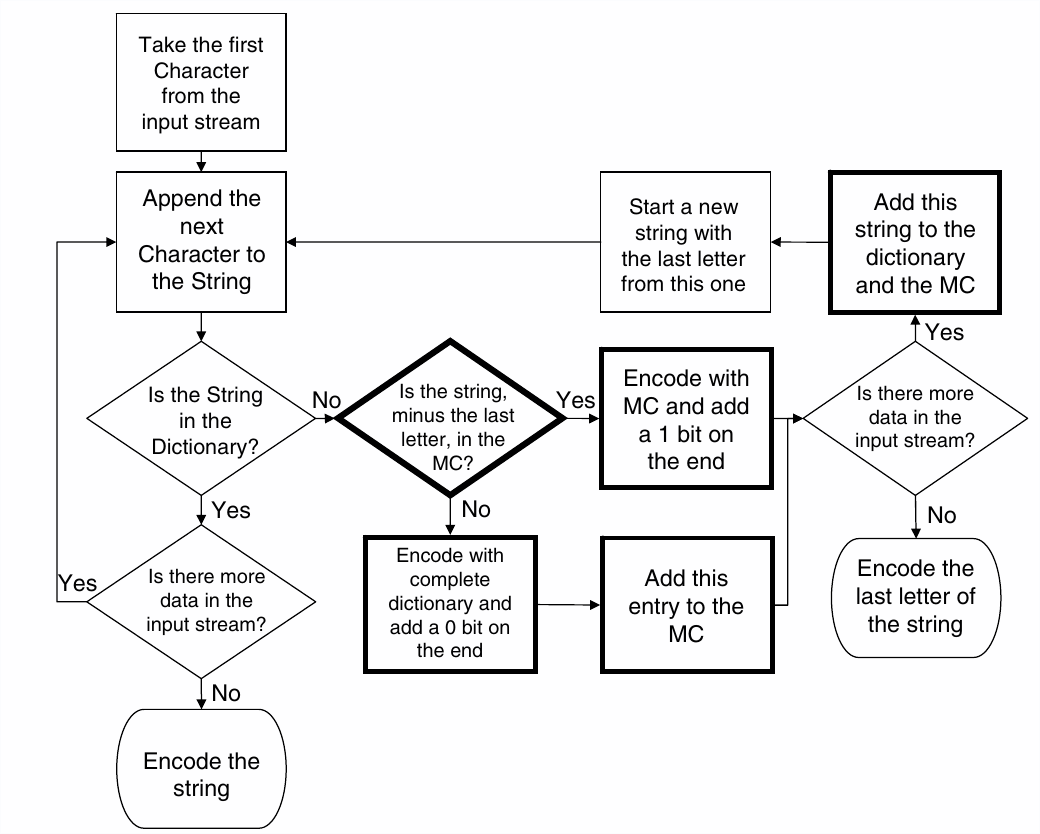
\includegraphics[width=\textwidth]{figures/S-LZW-MC.png}
    \caption{Flow chart of S-LZW-MC, extracted from~\cite{sadler2006data}}
    \label{fig:S-LZW-MC}
\end{figure}

By using Mini-Cache in S-LZW, the compression ratio improves, because of
representing data sequences by $O(\log N + 1)$ instead of $O(\log D)$,
where $N$ is the size of Mini-cache, $D$ is the size of the dictionary.
In~\cite{sadler2006data}, S-LZW offers energy savings, and it reduced
energy consumption on average by over 2.5$\times$.


\subsection{Lossless Entropy Compression Algorithm}

The Lossless Entropy Compression (LEC) algorithm was first proposed by
Marcelloni et al.~\cite{marcelloni2008simple}. It is a approximated version of
exponential-Golomb code~\cite{teuhola1978compression}. In
~\cite{marcelloni2008simple}, authors measured temperature and humidity by
sensors and compressed data by using LEC. It uses a very small dictionary whose
size is determined by the number of bits after analog-to-digital converter
(ADC)~\cite{marcelloni2008simple,marcelloni2009efficient}. For instance, in a
sensor node, a measure $m_i$ is gained and converted into numeral value $r_i$
represented using $R$ bits by ADC. For each new data point $r_i$, LEC compute
the difference of adjacent points $d_i$ = $r_i$ - $r_{i-1}$, in order to compute
$d_0$, the $r_{-1}$ equals the central value among $2^R$. The residue $d_i$ is
encoded by entropy encoder, and represented as a bit sequence in 2 parts $s_i |
a_i$ , where $s_i$ is a entropy code of $n_i$ which equals the value of the bits
needed to represent the difference $d_i$, and $a_i$ represent $d_i$ based on the
following rules:
\begin{enumerate}
    \item If $d_i = 0$, $a_i$ is not present.    
    \item If $d_i > 0$, $a_i$ is the binary expression of $n_i$ low-order bits
    of the $d_i$
    \item If $d_i < 0$, $a_i$ is the binary expression of $n_i$ low-order bits
    of the two's complement representation of ($d_i$ - 1)
\end{enumerate}

\noindent Where $n_i$ = 0 if $d_i$ = 0, else $n_i$ =
$(\log{_2}{\left|{b_i}\right|} + 1)$~\cite{li2016temporal} and $n_i \leq R$.

Table~\ref{table:LEC} is used for compression process
in~\cite{marcelloni2008simple, marcelloni2009efficient}. It supports R+1
groups($n_i$) and each group $s_i$ contains $2^{n_i}$ numeral value.
\begin{table}
\centering
\begin{tabular}{|l|l|l|}
\hline
$n_i$ & $s_i$        & $d_i$                                  \\ \hline
0     & 00           & 0                                      \\ 
1     & 010          & -1, +1                                 \\
2     & 011          & -3, -2, +2, +3                         \\
3     & 100          & -7, ..., -4, +4, ..., +7               \\
4     & 101          & -15, ..., -8, +8, ..., +15             \\
5     & 110          & -31, ..., -16, +16, ..., +31           \\
6     & 1110         & -63, ..., -32, +32, ..., +63           \\
7     & 11110        & -127, ..., -64, +64, ..., +127         \\
8     & 111110       & -255, ..., -128, +128, ..., +255       \\
9     & 1111110      & -511, ..., -256, +256, ..., +511       \\
10    & 11111110     & -1023, ..., -512, +512, ..., +1023     \\
11    & 111111110    & -2047, ..., -1024, +1024, ..., +2047   \\
12    & 1111111110   & -4095, ..., -2048, +2048, ..., +4095   \\
13    & 11111111110  & -8191, ..., -4096, +4096, ..., +8191   \\
14    & 111111111110 & -16383, ..., -8192, +8192, ..., +16383 \\
\hline
\end{tabular}
\caption{The dictionary used in LEC, reproduced from~\cite{marcelloni2009efficient}}
\label{table:LEC}
\end{table}
 
\subsection{Sequential Lossless Entropy Compression}

The Sequential Lossless Entropy Compression (S-LEC) algorithm is an extension
and improvement of LEC Algorithm by Li et al.~\cite{li2016temporal}. Similar to
LEC, it encodes residues in compression process, because adjacent residues
usually are not too large. In LEC, the result after encoding has two parts,
$s_i$ and $ a_i$, and the $s_i$ part contains information redundancy, if a set
of residues are in same group which means repeated group index $s_i$. S-LEC
reduces the size of representation by exploiting the correlation amount adjacent
residues. The main idea is using a extra two bits of sequential code $b_i$ to
present the positional relationship of groups of adjacent
residues~\cite{li2016temporal}. The encoding result $s_i|a_i$ is replaced by
$b_i|s_i|a_i$, but the group index $s_i$ is omitted if two adjacent residues are
in same group or neighboring group. Assume the number of the group in table is
K, then $b_i$ is defined as~\cite{li2016temporal}: 

\begin{enumerate}
    \item $b_i$ = 00, if $s_i$ = $s_{i-1}$
    \item $b_i$ = 01, if $n_i$ = $n_{i-1}$ - 1($n_{i-1} \geqslant 1$), or $n_i$
    = $n_{i-1}$ + 2($n_{i-1}$ = 0)
    \item $b_i$ = 10, if $n_i$ = $n_{i-1}$ - 1($n_{i-1} \leqslant K$), or $n_i$
    = $n_{i-1}$ - 2($n_{i-1}$ = K)
    \item $b_i$ = 11, otherwise. The representation $b_i|s_i|a_i$ is required. 
  \end{enumerate}

When the $b_i$ equals 11, the representation need more bits than LEC result,
because of extra $b_i$. S-LEC proposed some context situations to solve this
problem. In paper~\cite{li2016temporal}, the groups is divided into three
clusters: $C_1$ = {$n_i$|$i$ = 0, 1, 2, 3}, $C_2$ = {$n_i$|$i$ = 4, 5} and 
$C_3$ = {$n_i$|$i$ = 6, ..., K}. The idea of reducing group code as
follow~\cite{li2016temporal}:

\begin{enumerate}
    \item $s_i$ remove the first ``1'', If $n_{i-1} \in C_1$
    \item $s_i$ remove the first two ``1''s, If $n_{i-1} \in C_2$
    \item $s_i$ remove the first three ``1''s, If $n_{i-1} \in C_3$
\end{enumerate}
S-LEC gives better compression ratio than LEC when they have the same error
bound. We need to save the table into memory when we uses these two algorithms,
and in order to improve compression ratio as much as possible, it is necessary
to encode $n_i$ by prefix code method base on the elements distribution.

\TG{\#\#It would be useful to give an idea of the compression ratios and perhaps 
compute times provided by these algorithms}
